\section{Capstone: What a Per-Node MXU Feature Recovers}
\label{sec:capstone}

\subsection{A large gain at the shared learning rate}
\label{sec:capstone-shared}
% REVISE-IF-TIME: low 4-gram overlap with the First Draft.
We added one number to each convolution node, its channel-padding utilisation
(Section~\ref{sec:mxu}), and kept everything else identical to the flat baseline. The test set is
pre-registered: three convolution graphs (inception\_v3, resnet50.4x4.fp16, resnet\_v1\_50) on
xla:random and xla:default, with the four BERT and UNet graphs as a placebo. At lr 1e-3, convolution
Top-1 slowdown drops from 1.42 to 1.12, $\Delta = -0.30$ (Benjamini--Hochberg $p = .0032$, Cohen's
$d = -3.15$; Table~\ref{tab:arms}). The channel arm wins on all 6 graph--collection instances and on
all five seeds (Wilcoxon $p = .062$, the floor for five seeds), while the placebo graphs barely move
(1.0272 to 1.0292). The scramble control rules out extra capacity: shuffling the feature's values
between nodes keeps the input width but removes the information, and the real feature beats it
($\Delta = -0.244$, $p = .006$; rerun on matched GPU hardware, $-0.221$, $p = .003$). Spatial-only and
combined encodings also help, though the combined arm nudges the placebo graphs too. Before running
anything, we had predicted that the channel-only arm would not help; it was the strongest.

\begin{table*}[t]
\caption{Convolution (CONV, 3 graphs) and placebo (OTHER, 4 graphs) Top-1 slowdown for each MXU
encoding against the untuned baseline at the shared lr of 1e-3 (mean $\pm$ std over 5 paired seeds;
evaluation batch 32; verdicts unchanged at batch 8). BH-$p$ is Benjamini--Hochberg-adjusted over the
three arms.}
\label{tab:arms}
\centering
\small
% Generated by scripts/paper_figures.py from experiments/phase8c_results.json
\begin{tabular}{lccccc}
\toprule
Arm & CONV slowdown & OTHER slowdown & $\Delta$ CONV & BH-$p$ & $d$ \\
\midrule
baseline & 1.4246 $\pm$ 0.0721 & 1.0272 $\pm$ 0.0027 & -- & -- & -- \\
channel & 1.1203 $\pm$ 0.1077 & 1.0292 $\pm$ 0.0182 & -0.3043 & 0.0032 & -3.15 \\
spatial & 1.1758 $\pm$ 0.0389 & 1.0237 $\pm$ 0.0080 & -0.2488 & 0.0014 & -4.72 \\
full & 1.1933 $\pm$ 0.1479 & 1.0125 $\pm$ 0.0080 & -0.2313 & 0.0073 & -2.25 \\
\bottomrule
\end{tabular}

\end{table*}

\subsection{Against a tuned baseline, the gain is below detection}
\label{sec:capstone-tuned}
% REVISE-IF-TIME: low 4-gram overlap with the First Draft.
The baseline above is Section~\ref{sec:result1}'s handicapped arm: the same flat model at lr 1e-3,
which learns (overall $\tau = 0.2311$) but is undertrained, with 4 of 5 runs peaking at the final
epoch. A pre-registered check reran both arms over a grid of learning rates and kept each arm's best;
both landed on 3e-5, the lowest rate in the grid, so tuning may not have fully converged. Tuning alone
takes the baseline from 1.42 to 1.09, removing most of the convolution error. The channel feature's
remaining gain is $\Delta = -0.033$ ($p = .17$), below the five-seed MDE of 0.073. The tuned baseline
left so little room that no five-seed outcome could have reached significance under the registered
test. At evaluation batch 8 the gain is nominally significant ($-0.060$, $p = .045$), but the placebo
graphs move too ($p = .044$), and the registered batch is 32. This is the second instance of the
baseline-strength pattern.

\subsection{Robustness and generalisation}
\label{sec:capstone-robust}
The shared-rate result rests on three graphs from two families (Inception and ResNet). Dropping any one
graph still leaves a clear effect ($\Delta$ $-0.26$ to $-0.38$, all $p \leq .0099$; post hoc). On 19
instances from 6 convolution families the model never trained on, with both arms tuned, the gain points
the right way but is not significant ($\Delta$ $-0.11$, $p = .35$, MDE 0.39), and its direction flips
at evaluation batch 8. This test cannot say whether the feature generalises. Figure~\ref{fig:forest}
summarises every arm.

\begin{figure}[t]
\centering
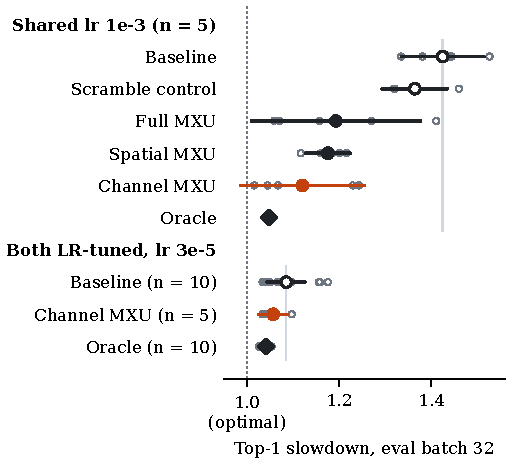
\includegraphics[width=\columnwidth]{figures/fig_k1_forest.pdf}
\caption{Convolution Top-1 slowdown per arm (mean, 95\% $t$-interval and seeds; evaluation batch 32;
1.0 = optimal). Top: at the shared lr of 1e-3, all three MXU encodings beat the baseline and the
scramble control. Bottom: with arms tuned at 3e-5, the baseline reaches 1.09 and neither the channel
feature nor the oracle is detectably better. The tuned baseline and oracle come from the 10-seed R5
run; the tuned channel arm comes from the 5-seed tuning check.}
\label{fig:forest}
\end{figure}

\subsection{The oracle ceiling}
\label{sec:oracle}
To bound how good a static model could get, we built an oracle that receives information derived from
the measured runtimes, so it cheats by design. At lr 1e-3 it reached 1.048, far ahead of the baseline,
with the channel arm in between. Our pre-registered prediction P5 required the oracle both to reach 1.05
and to beat the channel arm significantly; it reached the bar but not significance (gap 0.0725,
$p = .19$), so P5 is not confirmed. A power analysis done afterwards shows P5 could not have passed:
reaching 1.05 capped the oracle's possible advantage at 0.0703, below the five-seed MDE of
0.091--0.116, and the observed gap would have needed about 18 seeds. At evaluation batch 8 the gap is
significant ($-0.099$, $p = .020$), but the registered batch is 32. Our own pre-registration fell into
the under-powering trap that Section~\ref{sec:audit} describes.

We then re-ran the oracle against a tuned baseline, choosing 10 seeds by a power check before running.
At the registered batch 32, the oracle's lead is not detected ($\Delta$ $-0.043$, $p = .056$, MDE
0.062); at batch 8 it is significant in the same direction ($\Delta$ $-0.093$, $p = .003$). On the
placebo graphs the oracle does slightly worse than the baseline. Tuning barely moved the oracle but
moved the baseline a lot, so most of the headroom seen at 1e-3 came from the untuned baseline: the third
instance of the pattern. The lr-1e-3 oracle checkpoints all came from epoch 5 and were trained on CPU,
so the comparison between the two oracle runs is descriptive only.

\subsection{What remains open}
\label{sec:open}
Whether any convolution gap remains after tuning is unresolved at our seed count as the gap was
inconclusive (not detected) at batch 32 and only significant at batch 8. The registered reading of
this outcome is that label noise, which is the variation in measured runtimes from run-to-run, is
the deeper limit, but our test cannot separate label noise from information missing from the graph.
Answering the question would potentially need more seeds and more convolution graphs than three
graphs from two families.
